
%%%%%%%%%%%%%%%%%%%%%%%%%%%%%%%%%%%%%%%%%%%%%%%%%%%%%%%%%%%%%%%%%%%%%
%% This is a (brief) model paper using the achemso class
%% The document class accepts keyval options, which should include
%% the target journal and optionally the manuscript type.
%%%%%%%%%%%%%%%%%%%%%%%%%%%%%%%%%%%%%%%%%%%%%%%%%%%%%%%%%%%%%%%%%%%%%
\documentclass[journal=ancham,manuscript=article]{achemso}

%%%%%%%%%%%%%%%%%%%%%%%%%%%%%%%%%%%%%%%%%%%%%%%%%%%%%%%%%%%%%%%%%%%%%
%% Place any additional packages needed here.  Only include packages
%% which are essential, to avoid problems later.
%%%%%%%%%%%%%%%%%%%%%%%%%%%%%%%%%%%%%%%%%%%%%%%%%%%%%%%%%%%%%%%%%%%%%
\usepackage{chemformula} % Formula subscripts using \ch{}
\usepackage{achemso}
\usepackage[T1]{fontenc} % Use modern font encodings
\usepackage{amsmath}
\usepackage{subfigure}
\usepackage{amsfonts}
\usepackage{multirow}

%%%%%%%%%%%%%%%%%%%%%%%%%%%%%%%%%%%%%%%%%%%%%%%%%%%%%%%%%%%%%%%%%%%%%
%% If issues arise when submitting your manuscript, you may want to
%% un-comment the next line.  This provides information on the
%% version of every file you have used.
%%%%%%%%%%%%%%%%%%%%%%%%%%%%%%%%%%%%%%%%%%%%%%%%%%%%%%%%%%%%%%%%%%%%%
%%\listfiles

%%%%%%%%%%%%%%%%%%%%%%%%%%%%%%%%%%%%%%%%%%%%%%%%%%%%%%%%%%%%%%%%%%%%%
%% Place any additional macros here.  Please use \newcommand* where
%% possible, and avoid layout-changing macros (which are not used
%% when typesetting).
%%%%%%%%%%%%%%%%%%%%%%%%%%%%%%%%%%%%%%%%%%%%%%%%%%%%%%%%%%%%%%%%%%%%%
\newcommand*\mycommand[1]{\texttt{\emph{#1}}}

%%%%%%%%%%%%%%%%%%%%%%%%%%%%%%%%%%%%%%%%%%%%%%%%%%%%%%%%%%%%%%%%%%%%%
%% Meta-data block
%% ---------------
%% Each author should be given as a separate \author command.
%%
%% Corresponding authors should have an e-mail given after the author
%% name as an \email command. Phone and fax numbers can be given
%% using \phone and \fax, respectively; this information is optional.
%%
%% The affiliation of authors is given after the authors; each
%% \affiliation command applies to all preceding authors not already
%% assigned an affiliation.
%%
%% The affiliation takes an option argument for the short name.  This
%% will typically be something like "University of Somewhere".
%%
%% The \altaffiliation macro should be used for new address, etc.
%% On the other hand, \alsoaffiliation is used on a per author basis
%% when authors are associated with multiple institutions.
%%%%%%%%%%%%%%%%%%%%%%%%%%%%%%%%%%%%%%%%%%%%%%%%%%%%%%%%%%%%%%%%%%%%%
\author{Valeria Fonseca Diaz}
\email{valeria.fonsecadiaz@kuleuven.be}
\author{Bart De Ketelaere}
\email{bart.deketelaere@kuleuven.be}
\author{Ben Aernouts}
\email{ben.aernouts@gmail.com}
\altaffiliation{Biosystems TC, KU Leuven,
Kleinhoefstraat 4, Geel, Belgium}
\author{Wouter Saeys}
\email{wouter.saeys@kuleuven.be}
\affiliation[KU Leuven]
{KU Leuven, Kasteelpark
Arenberg 30, Leuven, Belgium}
%%%%%%%%%%%%%%%%%%%%%%%%%%%%%%%%%%%%%%%%%%%%%%%%%%%%%%%%%%%%%%%%%%%%%
%% The document title should be given as usual. Some journals require
%% a running title from the author: this should be supplied as an
%% optional argument to \title.
%%%%%%%%%%%%%%%%%%%%%%%%%%%%%%%%%%%%%%%%%%%%%%%%%%%%%%%%%%%%%%%%%%%%%
\title[An \textsf{achemso} demo]
  {On unsupervised sample selection for multivariate calibration}

%%%%%%%%%%%%%%%%%%%%%%%%%%%%%%%%%%%%%%%%%%%%%%%%%%%%%%%%%%%%%%%%%%%%%
%% Some journals require a list of abbreviations or keywords to be
%% supplied. These should be set up here, and will be printed after
%% the title and author information, if needed.
%%%%%%%%%%%%%%%%%%%%%%%%%%%%%%%%%%%%%%%%%%%%%%%%%%%%%%%%%%%%%%%%%%%%%
%\abbreviations{IR,NMR,UV}
\keywords{sample selection, multivariate calibration, NIR, PLS}

%%%%%%%%%%%%%%%%%%%%%%%%%%%%%%%%%%%%%%%%%%%%%%%%%%%%%%%%%%%%%%%%%%%%%
%% The manuscript does not need to include \maketitle, which is
%% executed automatically.
%%%%%%%%%%%%%%%%%%%%%%%%%%%%%%%%%%%%%%%%%%%%%%%%%%%%%%%%%%%%%%%%%%%%%

% -----------------------------------------------------
% -------------------BEGIN DOCUMENT ------------
% -----------------------------------------------------

\begin{document}


% -----------------------------------------------------
% ------------------- abstract  ------------
% -----------------------------------------------------
\begin{abstract}
Indirect measurement of chemical composition through spectral measurements requires the establishment of multivariate calibration models. The reference analyses on the calibration samples typically form a major cost factor in the establishment of these multivariate models. Therefore, the aim of this study was to select the most informative calibration samples in an unsupervised way based on the spectral measurements. To this end, guidelines to address this challenge in PLSR model building has been developed which is defined on the basis of optimal sample size, input dimensionality and selection method. 

\end{abstract}%

% -----------------------------------------------------
% ------------------- introduction  ------------
% -----------------------------------------------------

\section{Introduction}\label{introduction}

Combination of spectroscopic measurements with multivariate calibration models has become the primary analytical tool to indirectly measure the chemical composition of products making processes such as those of quality control more cost-efficient. However, the practitioner still faces many challenges when building and maintaining these models. One main challenge involves the selection of the calibration samples for which reference analyses have to be performed. To provide guidance related to this, an exhaustive evaluation of the challenge of unsupervised sample selection to build successful calibration models has been investigated in this study. Within the range of applications of multivariate calibration, the stated problem is particularly relevant for indirect inspection of collected or observed natural samples using near-infrared (NIR) spectroscopy, which is common in the agrofood industry (AFI) \cite{Au2020,Diaz-Olivares2020, Saeys2005, Bobelyn2010}.  

As spectral measurements are easy and cheap to collect, a vast quantity of units can be submitted to these measurements with low effort. On the contrary, collecting the reference analyses is a task that requires substantial effort, high costs and possibly high waste. The challenge of unsupervised sample selection relates to determining the best methodology or strategy to select the samples that would be worthy of reference analyses (chemical composition values), based on spectral measurements to build calibration models.
This has been the motivation to pay attention to the optimization of model building costs while gaining model building effectiveness. Historically, the interpretation for this gain has been rephrased as the optimal spanning of variability with a minimum number of samples \cite{Naes1990, Saeys2019,Kennard1969}.

Because of the importance of this problem, optimal sample sizes and suitable strategies to select these samples have been active research domains for many years \cite{Ferre1996,Au2020, Liu2019}. Through the last decades, many methods have been proposed for sample selection within a finite set of units. Some of these have become widely accepted for their intuitively accurate approach and good performance \cite{Shetty2012a, Nawar2018, He2015}. The two most popular methods in the context of NIR spectroscopy and multivariate calibration are the Kennard-Stone\cite{Kennard1969} and  Puchwein\cite{Puchwein1988} algorithms. As a strategy, clustering techniques are widely accepted in order to account for multiple sources of variability\cite{Naes1990}, particularly when groups of samples exist in batches of collected products\cite{Bobelyn2010}. These popular algorithms have the common feature of relying on distance between the samples. Less popular in NIR applications but highly effective in product design are the D-optimal experimental designs, which translate the concept of variability from distance between samples to the variance of the coefficients of an assumed model \cite{Goos2011}. Yet, no clear understanding exists about which of all these methods are more suitable for NIR applications with multivariate calibration and no exhaustive competition of them has been disseminated to the knowledge of the authors. The most recent study found related to this problem used a selection method similar to the Puchwein algorithm and random selection to build models for the prediction of available nitrogen and total formylated phloroglucinol compounds in Eucalyptus leaves\cite{Au2020}. In the mentioned work, some guidelines were provided for the current problem, such as starting with a low number of samples and analyze the crossvalidation error in order to decide whether more samples are needed to better train the calibration model. In addition, absolute values about the required sample size were found, such as 200 samples for the prediction of available nitrogen\cite{Au2020}.

Multivariate calibration is a concept that in principle can involve any type of statistical model. Moreover, calibrations are made for classification as well as regression tasks \cite{Saeys2019}. While the present work focuses on regression models, the guidelines presented here can also serve as a criterion for classification model building. Regarding the model architecture, the effectiveness of the type of bilinear models that are widely used for NIR applications has been reported by many researchers. Unless the spectral values have a strong nonlinear relationship with chemical reference values, bilinear models such as partial least squares regression (PLSR) or principal component regression (PCR) remain the workhorse model architectures. Most of the work that can be found addressing the current problem of interest provides answers about the minimum required sample size using PLSR models \cite{Naes1990, Au2020, Shetty2012a, Rodionova2008}. However, the diversity in the answers may rather confuse researchers than provide clear guidance. 

Therefore, the aim of this study was to provide a structure approach for the selection of calibration samples by understanding the properties of PLSR models. The general framework of statistical learning theory proposed by Vapnik provides specific guidelines for the sample size needed depending on the model architecture to be used\cite{Vapnik2019, Vapnik2000}. In order to apply these rules to multivariate calibration of spectroscopic sensors, PLSR has to be positioned within the framework explained by Vapnik. In a similar way, to understand the required features to take into account for a successful PLSR model, it is essential to seek for the elements of the PLSR architecture that can be controlled with unsupervised measurements. In the remainder of this article, these aspects will be described and explained for the state-of-the-art methods to select calibration samples.

A general and a specific framework of PLSR is presented in order to set a context of analysis to solve the problem of the best strategy for unsupervised sample selection. The work is organized as follows. First, a description of the general and specific frameworks is presented as a basis to define the research questions of the current work. Next, the experimental work and results are presented along with the discussion of the aspects that lead to a more successful unsupervised sample selection to build calibration models. This will culminate in a schematic guideline for efficiently selecting calibration samples. Finally, conclusions will be drawn and suggestions for future research will be presented.

% -----------------------------------------------------
% ------------------- frameworks  ------------
% -----------------------------------------------------

\section{Frameworks to describe properties of PLSR}

\subsection{Statistical learning theory as a general framework}

Statistical learning theory, as proposed by Vapnik\cite{Chapelle2002}, provides a general framework for analyzing the properties of PLSR. While PLSR has been presented as a particular case of the derived continuum regression \cite{Stone1990}, it was not found to be positioned within the current proposed framework. From the perspective of Vapnik, in the general regression task, the response variable is assumed to be a linear combination of basis functions plus an error variable. With that model architecture and using a quadratic loss, the objective to estimate the model is to minimize the squared error \cite{Chapelle2002}. More concretely, let $y \in \mathbb{R}$ be the random variable representing the chemical constituent of interest and  $\mathbf{x} \in \mathbb{R}^{p}$ the predictor vector of spectral measurements. The regression model is defined as $y = f(\mathbf{x}, \boldsymbol{\beta}) + \epsilon$.  The general least squares regression problem can be established as \cite{Chapelle2002}:

\begin{equation}
    \min E \left[ (y-f(\mathbf{x}, \boldsymbol{\beta}))^2\right]; \quad f(\mathbf{x}, \boldsymbol{\beta}) = \sum_{k=1}^{\infty} \beta_k \phi_{k}(\mathbf{x})
    \label{eq_general_regression_problem}
\end{equation}

where $\{\phi_{i}(\mathbf{x})\}$ constitutes a basis of $L_2$ for which its elements can be ordered by some criterion. In the context of statistical learning theory by Vapnik, $E \left[ (y-f(\mathbf{x}, \boldsymbol{\beta}))^2\right]$ is called the \emph{expected risk}, which in practice is replaced by the designated \emph{empirical risk} in the presence of a set of $n$ observations to estimate function $f$ \cite{Vapnik2000}. This empirical risk is calculated as the sum of squared errors. The important feature of this optimization task is that to ensure a small \emph{expected risk}, the \emph{empirical risk} should be minimized over a limited number of basis functions $\{\phi_{k}(\mathbf{x})\}_{k=1}^d$. Therefore, the regression problem becomes:

\begin{equation}
    \min \frac{1}{n} \sum_{i=1}^n (y_i-f_d(\mathbf{x}_i, \boldsymbol{\beta}))^2; \quad f_d(\mathbf{x}, \boldsymbol{\beta}) = \sum_{k=1}^{d} \beta_k \phi_{k}(\mathbf{x})
    \label{eq_square_loss_empirical_regression_problem}
\end{equation}

It is in this regard that the problem stated in eq. (\ref{eq_square_loss_empirical_regression_problem}) corresponds to the definition of the PLSR model  \cite{Stone1990}, where the basis $\{\phi_{k}(\mathbf{x})\}$ is constructed by maximizing the covariance between $y$ and $\mathbf{x}$. The order in this basis is established by the covariance deflation at each step of the PLSR algorithm. The key element in this framework is the fact that the number of chosen basis functions $d$ corresponds to the so-called $VC$ dimension in Vapnik's theory, which measures the capacity control of a learning machine \cite{Vapnik2019}. The importance of the capacity control parameter $d$ is that it serves as the reference for determining a suitable sample size when aiming to build a regression machine, or, in the context of chemometrics, a multivariate calibration model. In the work by Vapnik, it has been stated that the ratio between the sample size and the $VC$ dimension determines whether the sample size is large or small. As the sample becomes large, the \emph{empirical} risk becomes closer to the \emph{expected} risk \cite{Vapnik2000}. Although there is no absolute threshold, it has been stated that the sample size is considered \emph{large} when  $n/d>20$ \cite{Vapnik2000}.


\subsection{Multivariate calibration as a specific framework}

In multivariate calibration, the basis of $L_2$ is what is known as the set of latent variables. Based on a set of $n$ observations stored in the matrices $\mathbf{X}_{n\times p}$ and $Y_{n\times 1}$, the underlying idea of the PLSR algorithm is to calculate latent variables $\{\phi_{k}(\mathbf{x})\}$ such that $\phi_k(\mathbf{x}) = \mathbf{Xv}_{k}$, where $\mathbf{v}_k$ results from maximizing the covariance between $\mathbf{X}$ and $Y$ at the $k$-th deflation step \cite{DeJong1993}. 

For a given value of $d$, the set of resulting latent variables constitute a set of orthonormal variables $\{\phi_{k}(\mathbf{x})\}_{i=1}^d$. However, the set of loading vectors $\{\mathbf{v}_k\}$ is defined as $\mathbf{S}$-orthogonal, given that $\mathbf{v}_k'\mathbf{S}\mathbf{v}_j = 0 \quad (j<k)$, where $\mathbf{S}$ is the covariance matrix of $\mathbf{X}$. The $\mathbf{S}$-orthogonality property of the PLSR algorithm indicates that the estimation of this type of regression model depends highly on the covariance matrix $\mathbf{S}$. This property suggests that if $n<N$ samples are found such that $\mathbf{S}_n$ and $\mathbf{S}_N$ are equivalent, there is no pure unsupervised information discarded that serves the PLSR model in the $N-n$ remaining samples.

There are several methods and indexes to study the equivalence between two matrices \cite{Tomic2013}. For the sake of bilinear regression models such as PLSR, it becomes manifest to evaluate this equivalence via the eigendecomposition (ED) of the matrices due to the rank deficiency of $\mathbf{S}$ in spectroscopy applications. Two criteria to quantify the equivalence arise from the ED. On the one hand, two matrices with the same eigenvectors are regarded as congruent matrices, which is a type of equivalence relationship\cite{Horn1985}. On the other hand, as the ED of $\mathbf{S}$ constitutes the theory of principal component analysis (PCA), the eigenvalues of $\mathbf{S}$ account for the variability that the individual dimensions contain and their relative predictive power for a regression model \cite{Artemiou2013}. Thus, the variability explained by two matrices can be compared based on their eigenvalues. Although this comparison directly relates to principal component regression (PCR), the present work focuses on the role of matrix $\mathbf{S}$ in PLSR models.

% -----------------------------------------------------
% ------------------- research questions  ------------
% -----------------------------------------------------

\section{Research questions}

The present work aims at presenting a systematic approach to the problem of unsupervised sample selection for PLSR model building. This scheme is defined in terms of three factors, namely, selection methods, the dimensionality of the matrix $\mathbf{S}$ and sample size to obtain calibration models with satisfactory performance. The objective is to provide answers to the following research questions:

\begin{itemize}

    \item Can a particular threshold be found regarding the optimal sample size for satisfactory PLSR models in chemometrics based on the ratio $n/d$?

    \item What is the effect of input dimensionality, sample size and selection method on the equivalence between $\mathbf{S}_N$ and $\mathbf{S}_n$?
    
    \item What are the most optimal conditions of the three factors for satisfactory PLSR models?

\end{itemize}

% -----------------------------------------------------
% ------------------- experimental  ------------
% -----------------------------------------------------

\section{Experimental}\label{experimental}

\subsection{Case studies}\label{data}

Two case studies from the agrofood industry were used to demonstrate the previously discussed aspects about unsupervised sample selection. From a wide range of cases, the current ones were chosen to demonstrate the effect of sample selection strategies for chemical constituents that can be easy or hard to predict. Other selection criteria were the total number of samples in each data set and the availability of an independent test set. 

The first case corresponds to the inspection of milk composition where data from two time periods were available both for spectral signals and reference analysis \cite{Diaz-Olivares2020}. During the first period, 316 samples were collected, while 79 new samples were collected in the second period. The time frame between the periods was two weeks. The spectral measurements correspond to transmittance mode acquired in the 900 nm - 1700 nm range with a resolution of 3 nm. In this case, the chemical constituent of interest was lactose, which has been shown to be more difficult to predict than the fat or protein content\cite{Aernouts2011}.

The second case involves NIRS on pig manure samples to measure the composition \cite{Saeys2005}. One set of 420 samples was measured for calibration and a second set of 164 samples was measured for validation. Calibration models were built for dry matter content, which has been shown to dominate the NIR spectra. The spectra were acquired in reflectance mode in the 426 nm - 1686 nm range with a resolution of 9 nm.

To clarify the terminology, the sets from which samples are to be selected will be referred to as original sets and the selected samples from the original sets will constitute calibration sets. The descriptive statistics of the data sets are summarized in Table \ref{tab_descriptive_statistics}.

\textbf{Preprocessing:} Mean centering preprocessing was used in all cases. Initial experiments were carried out to decide whether to preprocess the data with other specific filters, but this gave unsatisfactory results in the sample selection. It was observed that assuming certain preprocessing filters for the spectral measurements prior to any knowledge of the $y$ values may be harmful to the subsequent calibration models. 

\begin{table*}[t]
\centering
\begin{tabular}{|c|c|c|c|c|} 
\hline
Case study	& set & size & mean($y$) & std($y$)  	\\
\hline
\multirow{2}{10em}{Milk ($y$: lactose (\%))} & original set & 316 & 4.7371 & 0.1547\\
& test set & 79 & 4.7044 & 0.1554\\
\hline
\multirow{2}{10em}{Manure ($y$: dry matter ($gl^{-1}$))} & original set & 420 & 66.0224 & 34.7173\\
& test set & 164 & 64.2887 & 38.5147 \\
\hline 


\end{tabular}
\caption{Descriptive statistics}
\label{tab_descriptive_statistics}
\end{table*}

\subsection{Methodology}\label{methodology}

\subsubsection{Exhaustive evaluation}

An exhaustive evaluation was set up combining three main factors involved into sample selection. For each calibration set selected from the original set, the equivalence between covariance matrices was calculated and a PLSR model was built and applied on the test set. This allowed to evaluate the impact of the factors on model performance and on the resulting equivalence between covariance matrices. 


\subsubsection{Factors for unsupervised sample selection}

Three main factors involved in the problem of interest were considered: Method, input dimensionality and sample size. The definition of each factor is explained below and their possible values are listed in Table \ref{tab_samplesel_settings_exhaustive_search}. A calibration set was selected for each possible combination of the three factors.

\textbf{Selection methods}

A wide range of methods has been proposed for sample selection based on the available matrix $\mathbf{X}$. Based on a review of literature on chemometrics and calibration models, the following methods were selected: Kennard Stone (KS) \cite{Kennard1969}, Duplex (DUP) \cite{Snee1977}, Puchwein (PUCH)\cite{Puchwein1988}, complete linkage hierarchical clustering (CL) \cite{Naes1990} and D-optimal designs based on the Federov algorithm (D-OPT) \cite{Goos2011}. In addition, random selection (RAND) was included  as a benchmark to quantify the added value of the other methods. These methods have been adopted as standard methods for unsupervised sample selection in the context of chemometrics, proving good performance for calibration model building and serving in many research works in the last decades \cite{Naes1990, Brandmaier2012, Saeys2019, Au2020, Aernouts2011}.

The KS method selects the most central sample in the original set and then iteratively selects the sample that is the farthest from the selected sample(s). For a set of $k$ selected samples, the distance of each remaining sample is the maximum distance from the sample to each selected sample \cite{Kennard1969}. The calibration set is obtained after selecting the desired $n$ samples.

The DUP method aims to split the data set into two equal subsets. It starts by selecting the two farthest points in the original set to be placed in group 1 and then selects a second couple of two farthest points to be placed in group 2. From there, iteratively, the next point from the remaining samples that is the farthest from group 1 is assigned to this group and the same for group 2. When $n$ is reached in one of the groups, this group is taken as the calibration set \cite{Snee1977}.

PUCH is regarded as a type of clustering algorithm in which the selected points are representative for a neighborhood of points. The first selected point of the original set is the one farthest from the center. A neighborhood of samples for this point is detected given a limiting distance and they are discarded. Iteratively, the procedure continues by selecting the next farthest point from the center of the available samples and discarding its neighborhood. The selection ends when there are no more samples available and the selected points constitute the calibration set. In this study, the limiting distance was set according to the desired sample size $n$ \cite{Puchwein1988}.

CL consists in building the hierarchical clustering structure with complete linkage on the original set, which states that the distance between two clusters is the maximum pairwise distance of its members. The structure is cut at the number of clusters corresponding to the desired sample size $n$ and the selected points in the calibration set are the most central points of each cluster \cite{Naes1990}.

D-OPT is a type of experimental design that relies on a regression model aiming to maximize the determinant of the covariance of the model matrix. The model matrix includes several types of \emph{effects} calculated from the input variables of the model. The most basic model is one that includes the so-called \emph{main effects} which correspond to the values of the input variables. Higher-order effects can also be included which are polynomial orders of the input variables. The effects to be included depend on the purpose of the regression model for the response variable \cite{Goos2011}. For sample selection, the Federov algorithm selects a random initial design of size $n$. Next, it interchanges samples from the current design and the remaining original set until the determinant of the covariance of the model matrix is maximal. The resulting points of the design constitute the calibration set. Because the initialization of this algorithm is random, the available implementation of the algorithm takes multiple starting designs and delivers the convergent design \cite{Wheeler2019}.


\textbf{Input dimensionality}

The available spectral measurements stored in matrix $\mathbf{X}_{N\times p}$ have as input dimensionality $p$. However, due to the rank deficiency of $\mathbf{X}$, which is equivalent to the rank deficiency of $\mathbf{S}$, the input dimensionality was taken as the second factor involved in the sample selection. For an input dimensionality $a$, the samples were selected using the PCA scores $\mathbf{T}_{N\times a} = \mathbf{X}_{N\times p}\mathbf{R}_{p\times a}$ where $\mathbf{R}_{p\times a}$ contains the first $a$ eigenvectors of $\mathbf{S}_N$. Based on the evaluation of the current cases and results reported in the chemometrics literature, the range of $a$ was set from 1 to 25. In addition, the selection based on the original matrix $\mathbf{X}_{N\times p}$ was included as a benchmark to quantify the added value or reducing the dimensionality. This feature is referred to as $a=p$. The value of $a$ should not be confused with the $VC$ dimension for the PLSR model $d$. 

\textbf{Sample size}

Based on the maximum number of principal components ($a=25$), the minimum sample size was set to 30 samples in order to leave a small margin. The sample size range was considered in steps of 10 from 30 to the maximum number of samples available in the original set for each case study. 

\textbf{Constraints}

For the distance-based selection methods (KS,DUP,PUCH,CL), a Mahalanobis distance was used for $a=1,...,25$.  For $a=p$ a Euclidean distance was used, because the inverse of the covariance matrix $\mathbf{S}$ used in the Mahalanobis distance becomes unstable in this case. For the same reason, the selection based on D-OPT could only be applied for $a=1,...,25$. 

\begin{table*}[t]
\centering
\begin{tabular}{|r|l|} 
\hline
Selection method & KS, DUP, PUCH, CL, D-OPT, RS\\
\hline
Input dimensionality $a$ & 1, 2, ... , 25, $p$ \\
\hline
Sample size $n$ & 30, 40, ... , $N$ \\
\hline

\end{tabular}
\caption{Sample selection settings}
\label{tab_samplesel_settings_exhaustive_search}
\end{table*}

\subsubsection{Equivalence analysis of covariance matrices $\mathbf{S}_n$ and $\mathbf{S}_N$}

For the original set and a given calibration set, the equivalence between the covariance matrices $\mathbf{S}_N$ and $\mathbf{S}_n$ was evaluated through the correspondence of their eigenvectors and the eigenvalues. For this, the eigendecomposition (ED) of the matrices $\mathbf{S}_N = \mathbf{V}_N \mathbf{\Delta}_N \mathbf{V}'_N$ and $\mathbf{S}_n = \mathbf{V}_n \mathbf{\Delta}_n \mathbf{V}'_n$ was calculated. The rank of these decompositions was set to the value $a$ with which the calibration set was selected. The eigenvalues were compared by calculating the ratio  $\mathbf{\Delta}_n/\mathbf{\Delta}_N$ and the eigenvectors were compared by computing the absolute value of the determinant for the matrix $\mathbf{V}'_n\mathbf{V}_N$. As the set of eigenvectors constitutes also an orthonormal basis, this determinant takes an absolute value between 0 and 1. To avoid confusion, the terminology of PCA is used in the context of the input dimensionality explained previously, while the components of the current ED's are referred to as ED directions. 
In addition, in order to support the importance of the equivalence analysis, Pearson correlations between $y$ and the PCA scores were calculated.

\subsubsection{Multivariate calibration models}

The PLSR models were trained using the SIMPLS algorithm \cite{DeJong1993}.For each case study, PLSR models were built for all the selected calibration sets, which were then tested on the corresponding test set. The performance of the model was quantified as the root mean squared error in 10-fold crossvalidation (RMSECV) and for the test set (RMSEP) in a range for $d$ from 1 to 25 latent variables. 

\subsubsection{Computational tools}

The complete analysis was programmed in Python 3.7. The selection methods, excluding D-OPT, were programmed in house as well as the SIMPLS algorithm. The D-OPT method was used in a connection from R to Python, using the function \texttt{optfederov} from the R-package \emph{AlgDesign}\cite{Wheeler2019}. The exhaustive sample selection and subsequent PLSR calibrations were embedded into a loop which was highly optimized using \texttt{numba} for Python \cite{Lam2015}. It was possible to fit more than 5000 PLSR models including crossvalidation results in 10 minutes on an 64-bit Intel Core i7 vPro 8th generation with 16 GB of RAM. 


% -----------------------------------------------------
% ------------------- results  ------------
% -----------------------------------------------------

\section*{Results}\label{results}

\subsection*{Statistical learning theory as a general framework}\label{results:genframework}

\emph{Can particular thresholds be found regarding the optimal sample size for satisfactory PLSR models in chemometrics based on the ratio $n/d?$}

The model performance results for all the calibration models built in the exhaustive evaluation were put together in order to find a threshold for the optimal sample size regardless of the selection method or the input dimensionality. In total, 5360 models were built for the Milk case and 7210 models for the Manure case. For the current purpose, the optimal complexity $d$ for the prediction of lactose and dry matter needed to be established. Such an optimal complexity was chosen based on the minimum error in crossvalidation (RMSECV) using the original set and minimum error in prediction (RMSEP) using the test set, for each case study. Rather than fixing $d$ at a single value, a range of values for $d$ was chosen given the nearly monotonic behaviour of the error curves with increasing model complexity. 
Figure \ref{fig_d01_milk_general_framework}(a) shows the RMSE curves for lactose measurement in milk obtained in crossvalidation and test set prediction. Based on the above criteria, the optimal complexity was found between 16 and 18 \cite{Diaz-Olivares2020}. Therefore, to analyze the ratio $n/d$ using the lactose prediction, $d$ was set to 16, 17 and 18 latent variables. In the case of Manure, the same choices were made based on the RMSE curves shown in Figure \ref{fig_d02_manure_general_framework}(a). Because the two curves diverge from 11 latent variables onwards and the RMSECV becomes flat after 14 latent variables, the optimal complexity for DM was set to $d = 11,12,13 \text{ and } 14$\cite{Saeys2005}. 

Figures \ref{fig_d01_milk_general_framework}(b) and \ref{fig_d02_manure_general_framework}(b) show the RMSEP values as a function of the ratio $n/d$ for the chosen optimal complexities in each case study combining all the results from the exhaustive procedure. A clear stabilization of the prediction error as a function of the ratio of interest can be observed, regardless of the other factors for sample selection. For ratios below 10, there is large variability in the prediction performance of the models, which indicates that the sample size is too small compared to the optimal complexity of the calibration model. The prediction of the lactose content in milk stabilized for $n/d>12$, obtaining similar performance as reported in previous works\cite{Diaz-Olivares2020, Aernouts2011}. It should be noted that the number of samples in the original set (N=316) and the chosen optimal complexity accounted for a maximum ratio below 20. Interestingly, a similar trend can be observed in the prediction of the dry matter content in manure. A jump can be observed after a ratio of 12 and then a final stabilization point is reached for $n/d>16$ providing comparable performance as obtained in the reference work, provided that the data was only mean-centered in the current work\cite{Saeys2005}. In both cases, the highest variability in the performance of the calibration models was obtained for $n/d<10$. For these specific cases, this indicates that the model complexity of 16 latent variables required for accurate prediction of the lactose content in milk demands that the calibration set contains at least 16 *10 = 160 samples. As the optimal model complexity for predicting the dry matter content in manure required 11 latent variables, at least 110 calibration samples would be required.

\begin{figure}[b]
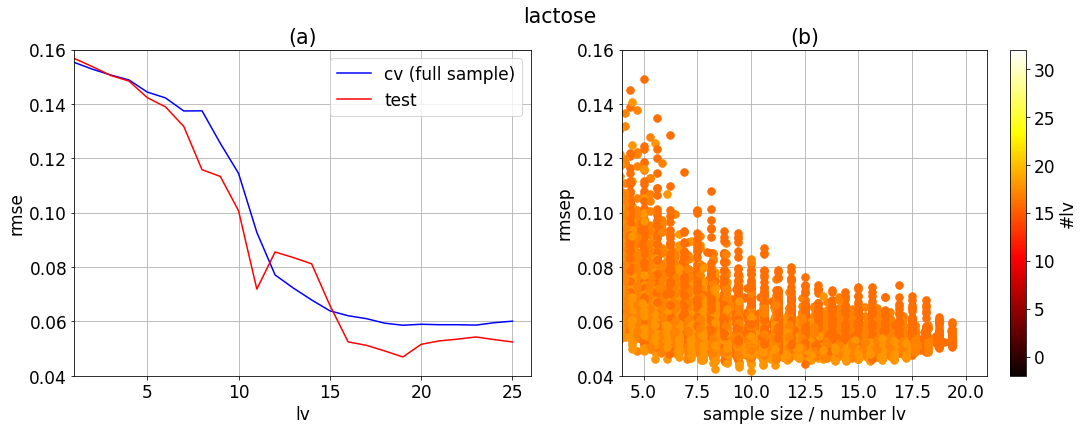
\includegraphics[width=0.8\textwidth]{manuscript/figures/d01_milk_general_framework.png}
\centering
\caption{Evolution of the error (RMSE) in predicting the lactose content in milk from NIR spectra as a function of (a) the number of latent variables $d$; and (b) the ratio of calibration samples over model complexity $(n/d)$ for $d$ values of 16 to 18.}
\label{fig_d01_milk_general_framework}
\end{figure}

\begin{figure}[b]
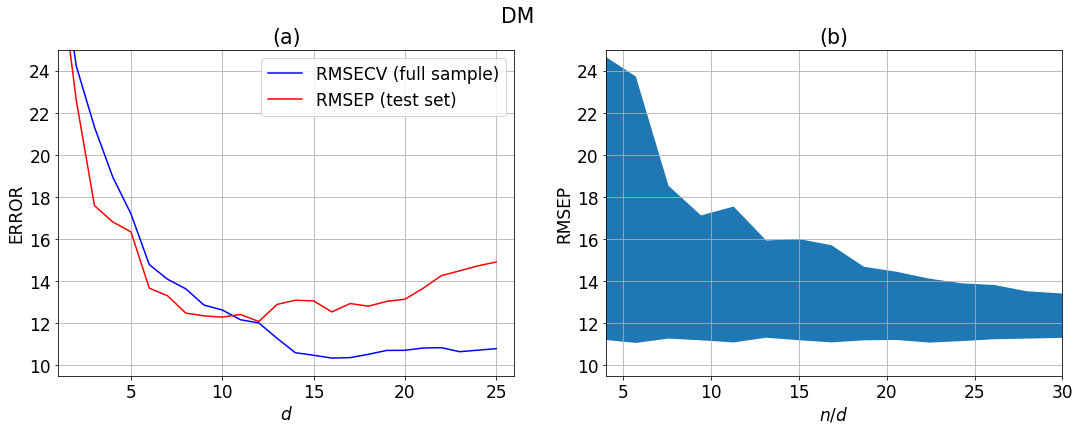
\includegraphics[width=0.8\textwidth]{manuscript/figures/d02_manure_general_framework.png}
\centering
\caption{Evolution of the error (RMSE) in predicting the dry matter content in manure from NIR spectra as a function of (a) the number of latent variables $d$; and (b) the ratio of calibration samples over model complexity $(n/d)$ for $d$ values of 11 to 14.}
\label{fig_d02_manure_general_framework}
\end{figure}

\subsection*{Multivariate calibration framework}\label{results:specframework}

\emph{What is the effect of input dimensionality, sample size and selection method on the equivalence between $\mathbf{S}_N$ and $\mathbf{S}_n$} 

As number of combinations of selection method, sample size and input dimensionality $a$ that has been evaluated is very large, the discussion on the degree of equivalence between $\mathbf{S}_N$ and $\mathbf{S}_n$ is limited to few discrete values of the input dimensionality $a$. The impact of the entire range of $a$ on the model performance is presented in the next section. Figure \ref{fig_specific_framework_detereigevect} shows the comparison of the eigenvectors of $\mathbf{S}_N$ and $\mathbf{S}_n$ for both case studies when the sample selection was made for $a=15$, 20 and 25 with each method. 

Across the different methods, the behavior of the determinant at a fixed $a$ was noticeably related to the sample size, yet differently for the different selection methods. Excluding DUP, all the other methods in both case studies showed similar results for $a=15$ and 20. Determinants above 0.8 were achieved with sample sizes below 30\% of N. When setting $a=25$ large differences were observed by the selected calibration sets across the different methods and sample sizes. In both case studies, CL and D-OPT selection showed a jump in the determinant around the same sample sizes. In the Manure case, KS related to CL and D-OPT in this behavior, while it was PUCH in the Milk case. As expected, due to the nature of selection with DUP creating two equivalent subsets, the determinant presents a decline after crossing 50\% of the samples for selection. However, this decline was obtained for $a=20, 25$ and not for $a=15$ indicating the effect of the input dimensionality. RAND selection did not achieve a clear stabilization of the determinant compared to that of the other selection methods.

For KS, PUCH, CL and D-OPT, the stabilization of the determinant for $a=25$ at a value of $n$ was in line with the threshold found with the ratio $n/d>12$. The comparison of the resulting individual eigenvalues is therefore presented for the selection made with $a = 25$ for both case studies in Figures \ref{fig_d01_milk_specific_framework_eigenvalsratio} and \ref{fig_d02_manure_specific_framework_eigenvalsratio}. Each curve represents the eigenvalues ratio for a given value of $n$. With the exception of DUP selection, there is a clear convergence towards 1 of these ratios as $n$ increases. This suggests that, ideally, a subset of samples could be selected such that the resulting eigenvalues are uniformly close to the eigenvalues based on the total number of samples. For small sample sizes, a high variation of the ratios occurred revealing that even when selecting the samples with $a=25$, not all dimensions are equally represented in the subset. Most interestingly, high peaks and drops happened at the same dimensions indistinctly of the selection method. As $n$ increases, the curves are flatter indicating an equitable representation of the individual dimensions. 

In this comparison, the 50\% effect of DUP selection was detected as the curves for the ratio of the eigenvalues was divided into 2 groups by 50\% of the samples. For $n$ bigger than 50\% in DUP, the variability starts being underestimated as the curves drop below 1. In both case studies, KS, D-OPT and PUCH selection showed that there is generally no underestimation of variability as the eigenvalues ratio stayed above 1 with very few exceptions. No systematic behavior in the variability of the eigenvalues was revealed for RAND selection. 

As CL is a more robust method compared to the other methods in terms of control over possible outliers, the eigenvalues ratio is overall more stable and closer to 1 in comparison with the other methods. In the Milk case, for very small sample sizes, some dimensions resulted in ratios between 0.5 and 1. D-OPT showed more linearity for the eigenvalues ratio as a function of the sample size compared to the other methods in both case studies. 

\begin{table*}[t]
\centering
\begin{tabular}{|cc|cc|} 
\hline
\multicolumn{2}{|c|}{Milk (lactose)} & \multicolumn{2}{|c|}{Manure (DM)}\\
\hline
pc	& correlation	&  pc & correlation	\\
\hline
  1 & -0.1337 & 1 & -0.3132 \\
  2 & -0.1839 & 2 & -0.6231 \\
  3 & -0.0239 & 3 & -0.1587 \\
  4 &  0.2380 & 4 &  0.2220 \\
  5 &  0.0496 & 5 &  0.4036 \\
 16 &  0.0060 & 6 &  0.0299 \\
 17 &  0.0266 & 7 & -0.3102 \\
 18 &  0.4208 & 8 & 0.0521 \\
 19 &  0.1202 & 9 & 0.1543 \\
 20 &  0.0759 & 10& 0.0259 \\
 21 &  0.3819 &  & \\
 \hline
\end{tabular}
\caption{Pearson correlations between PC's and chemical component based on the selection set}
\label{tab_correlations}
\end{table*}

The possible risk of the non-uniform spanning of variability across the different dimensions was supported by the correlations between PC dimensions and the chemical constituent. Table \ref{tab_correlations} shows the Pearson correlations for both case studies. In the case of the Milk data set, PC's 18 and 21 showed higher correlations with lactose than PC's 1 and 2. In the Manure case, DM had a higher correlation with PC 5 than PC 1, but the first 10 PC's accounted for the highest correlations. The impact of diminishing or underestimating the variability at certain dimensions should thus be placed in perspective of the PLSR model performance in the next section. In regard to the equivalence between $\mathbf{S}_N$ and $\mathbf{S}_n$, the degree of equivalence depended on the rank value of $a$ and a more uniform span of variability according to the eigenvalues could be obtained in both case studies for sample sizes corresponding to $n/d>12$.  




\begin{figure*}[t]
    \centering
    \subfigure[Milk]{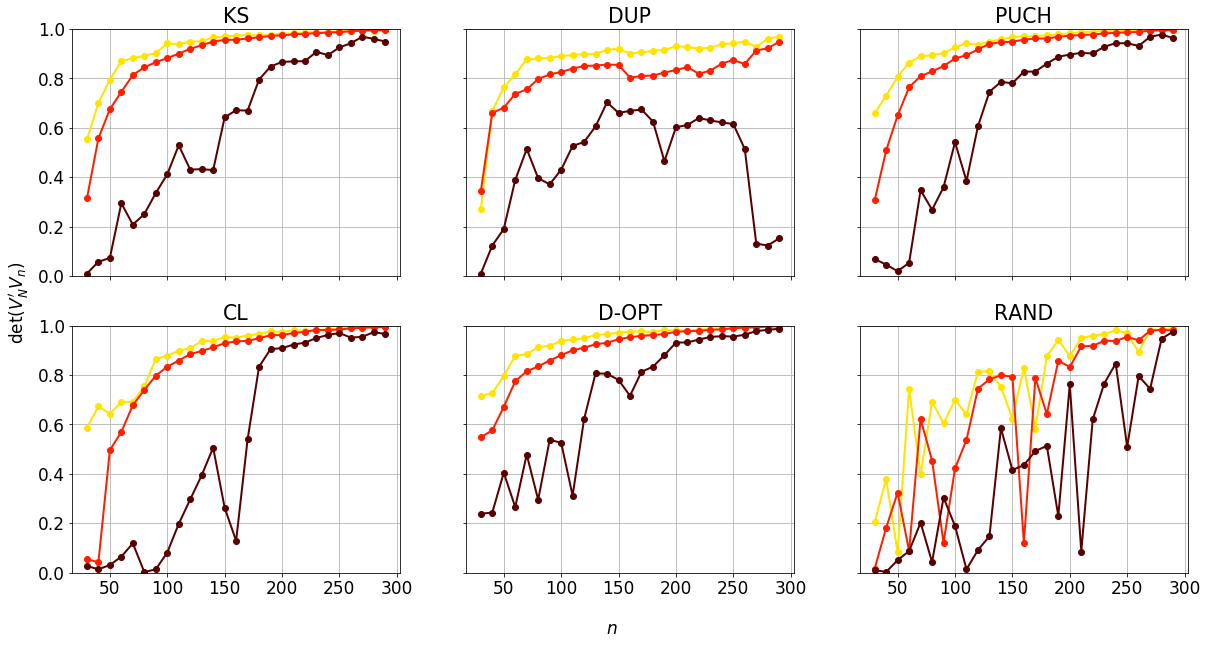
\includegraphics[width=0.6\textwidth]{manuscript/figures/d01_milk_specific_framework_detereigevect.png}} 
    \subfigure[Manure]{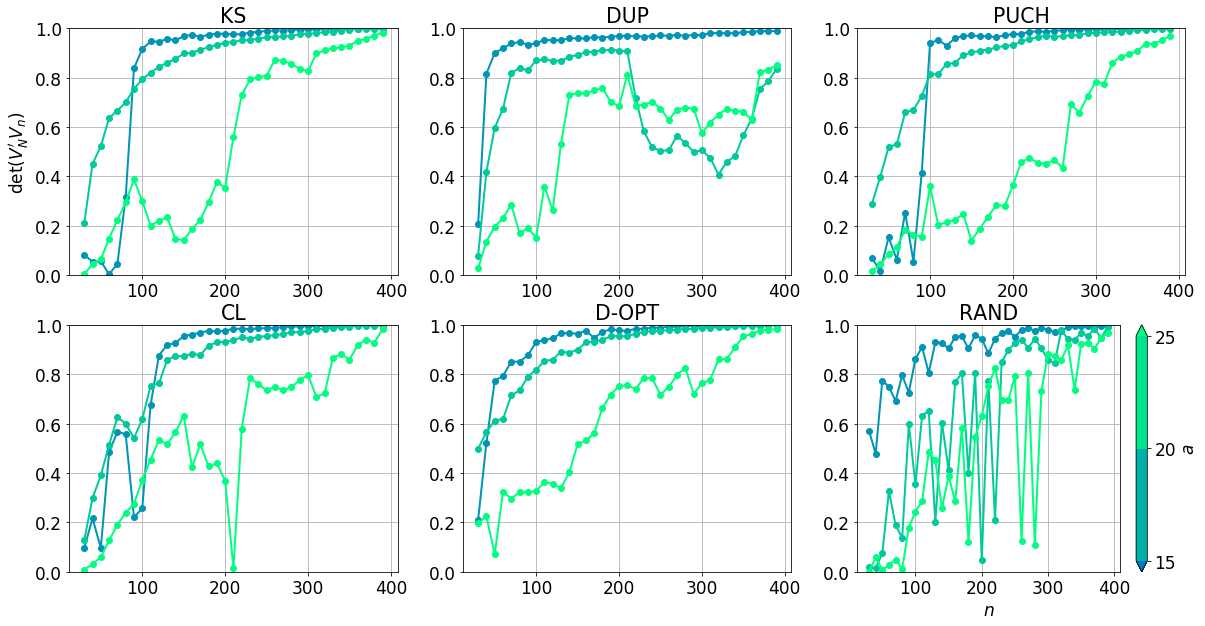
\includegraphics[width=0.6\textwidth]{manuscript/figures/d02_manure_specific_framework_detereigevect.png}}
    \caption{Comparison of eigenvectors when selecting samples with every method and input dimensionality $a=15,20,25$.}
    \label{fig_specific_framework_detereigevect}
\end{figure*}

\begin{figure}[b]
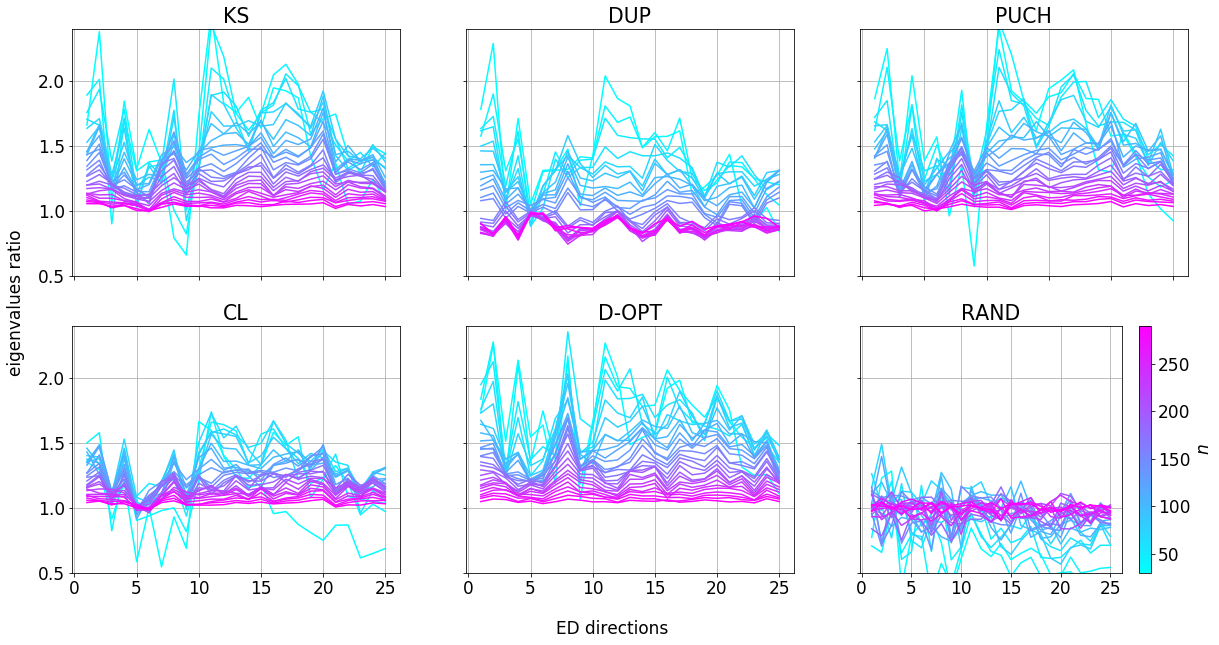
\includegraphics[width=0.8\textwidth]{manuscript/figures/d01_milk_specific_framework_eigenvalsratio.png}
\centering
\caption{Comparison of eigenvalues for Milk when selecting samples with every method and input dimensionality $a=25$.}
\label{fig_d01_milk_specific_framework_eigenvalsratio}
\end{figure}

\begin{figure}[b]
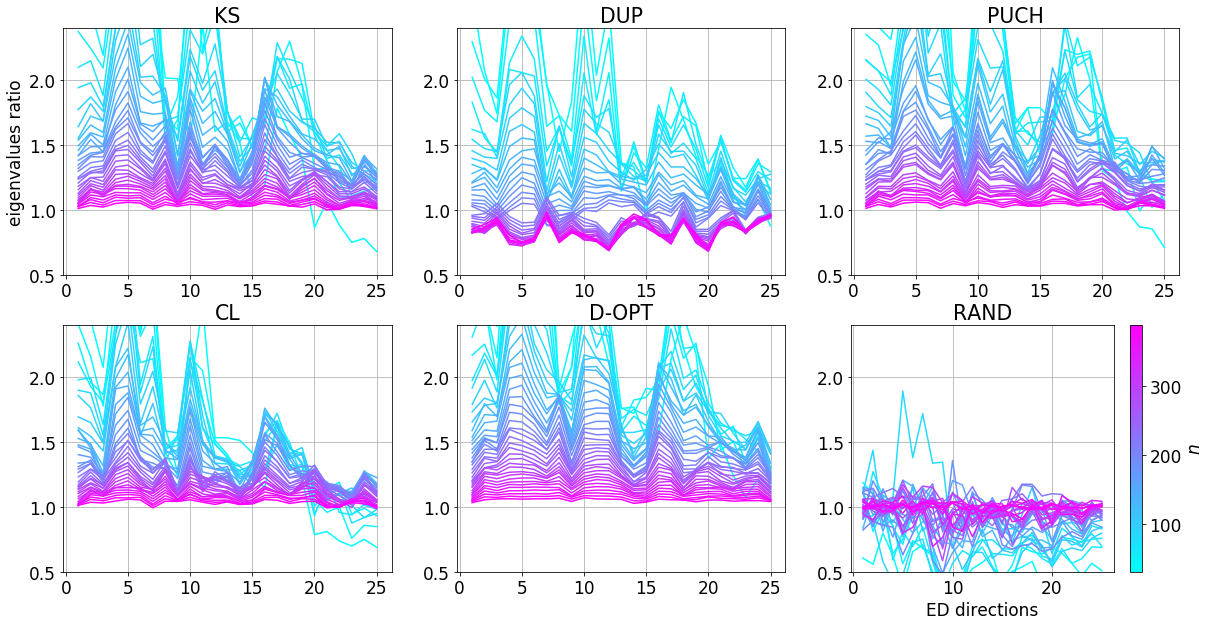
\includegraphics[width=0.8\textwidth]{manuscript/figures/d02_manure_specific_framework_eigenvalsratio.png}
\centering
\caption{Comparison of eigenvalues for Manure when selecting samples with every method and input dimensionality $a=25$.}
\label{fig_d02_manure_specific_framework_eigenvalsratio}
\end{figure}

\subsection*{Model performance}\label{results:modperformance}


\emph{What are the most optimal conditions of the three factors for satisfactory PLSR models?}

The simultaneous effect of the three selection factors on the performance of PLSR models was analyzed by comparing the RMSEP curves for each case study. The grid in Figures \ref{fig_d01_milk_model_performance} and \ref{fig_d02_manure_model_performance} shows the PLSR model performance for the Milk and the Manure case study, respectively. The selection methods are accommodated row-wise, punctual sample sizes are positioned column-wise and the color of the curves represents the input dimensionality. When comparing both case studies in terms of the impact of the sample selection factors, it can be concluded that the performance of the models with optimal complexity $d$ stabilized or converged for a sample size $n$ corresponding to the higher mentioned $n/d$ threshold of 12 for the optimal model complexity $d$.



\begin{figure}[b]
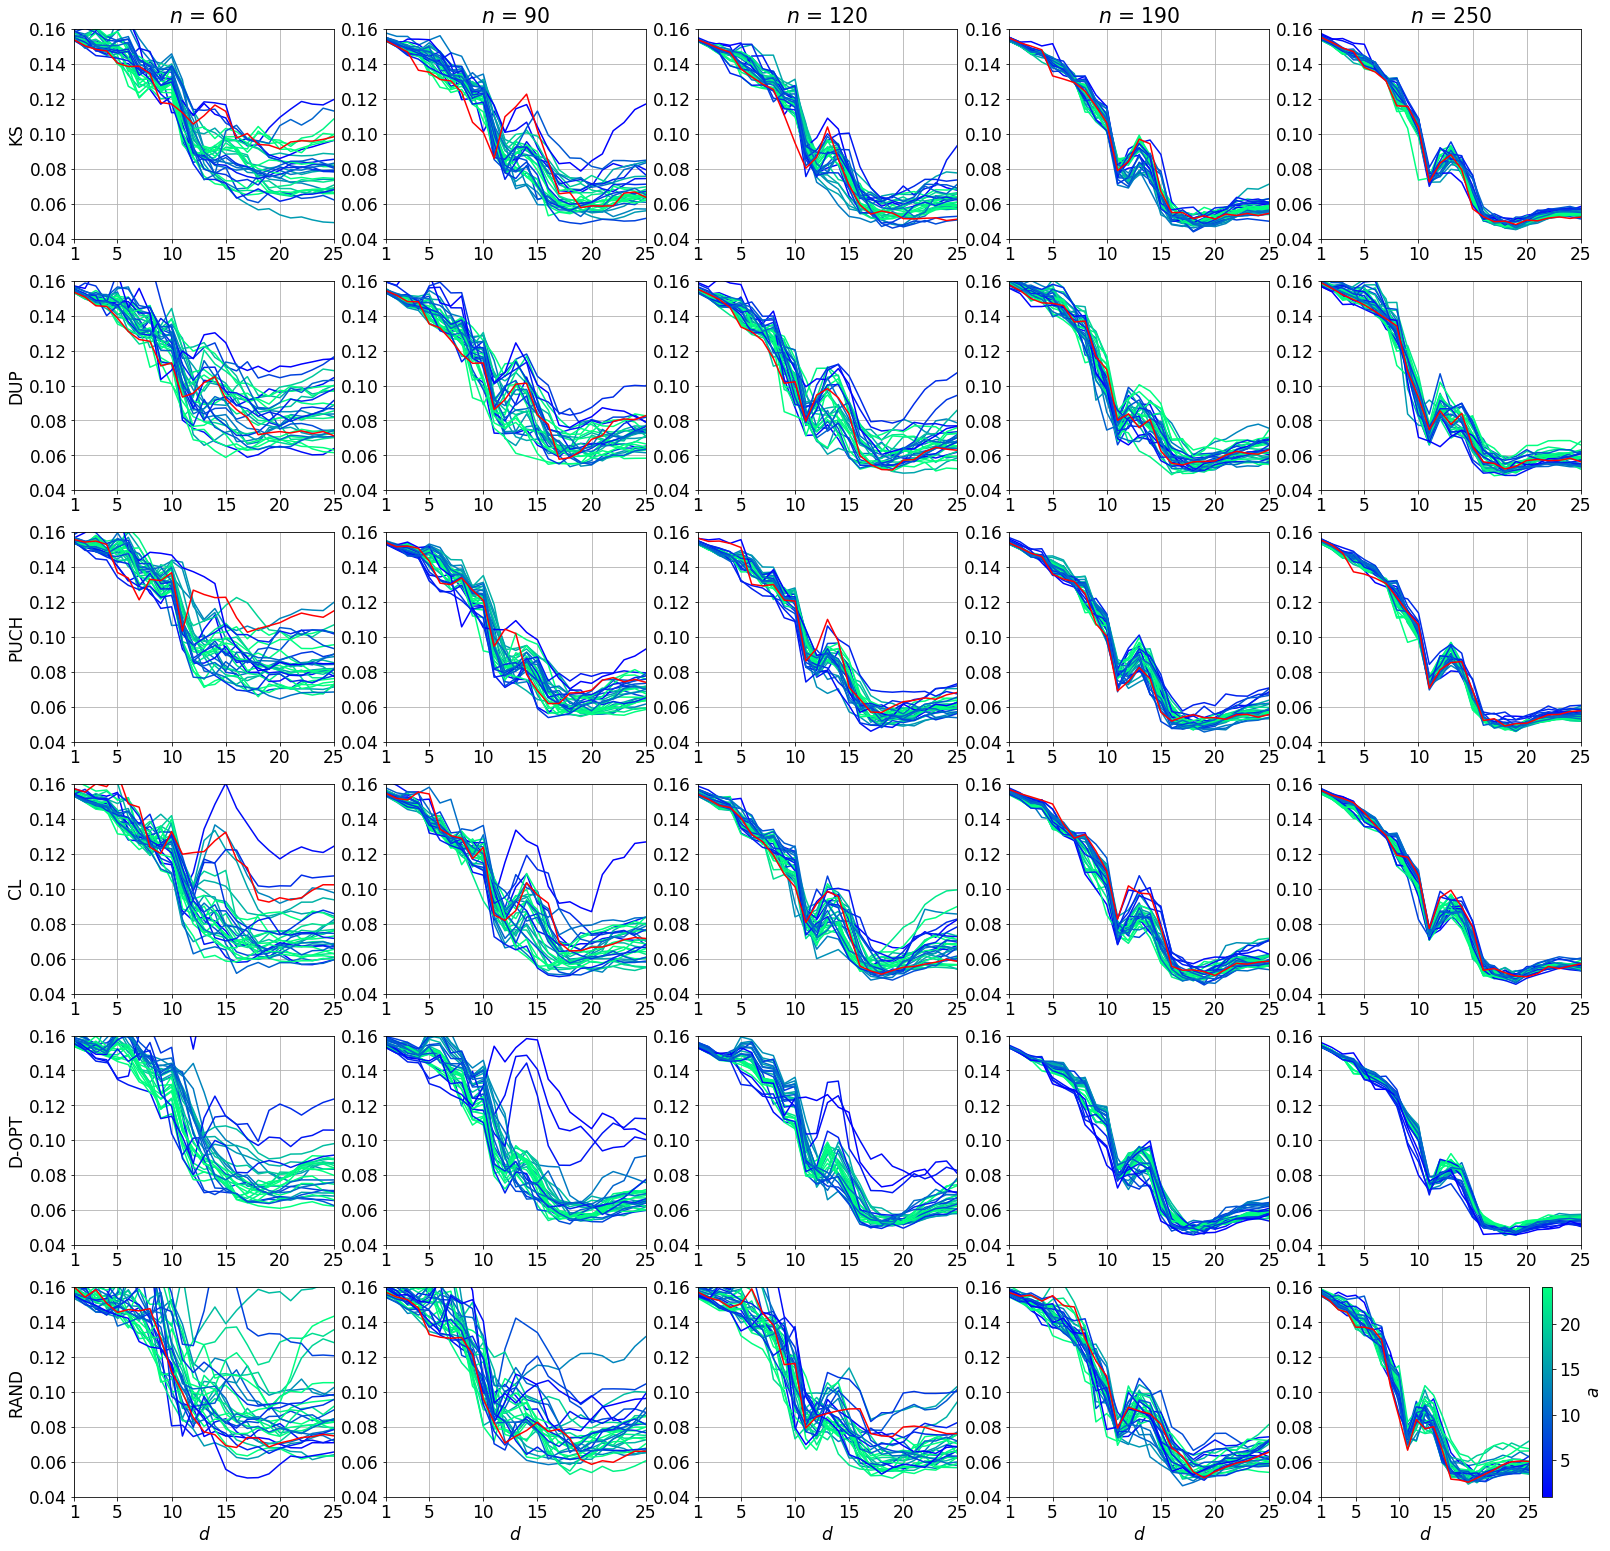
\includegraphics[width=0.8\textwidth]{manuscript/figures/d01_milk_model_performance.png}
\centering
\caption{Model performance to predict lactose according to selection method, input dimensionality and sample size. The red line represents input dimensionality $a=p$.}
\label{fig_d01_milk_model_performance}
\end{figure}

In both case studies, RAND selection resulted in larger variability in the model performance as the sample size decreased. For sample sizes as large as $n/d>16$, as revealed in the results of the general framework, RAND selection rendered calibration sets that were equally optimal as the sets delivered by any other selection method. In the prediction of lactose, the model performance for the selected sets of size $n=60$ was highly uncertain and no clear relation was found between a satisfactory performance and the selection method or the input dimensionality. Nonetheless, for such a small $n$, the selected set by D-OPT with a high value of $a$ consistently produced models with better performance than the other methods. Similar results were obtained with D-OPT for other small sample sizes ($n=90$ and $n=120$). This differentiation of the effect of the input dimensionality was not equally clear for small sample sizes with the other methods. Moreover, when selecting samples based on the original $\mathbf{X}$ matrix (i.e. $a=p$), there was no satisfactory result for the small sample sizes compared to values of $a$ between 15 and 25. When surpassing the threshold and selecting more than 160 samples, the performance of the models with the different methods and input dimensionality stabilized and no important or systematic difference was observed.

The model performances obtained for the Manure case suggest similar conclusions on the effect of the factors as in the Milk case study. In particular, for a small sample size $n=60$, D-OPT selection showed a more stable performance around $d = 11$ for large values of $a$ than the performance stability of the other methods. This stabilization by D-OPT was observed more clearly for $n=90$ from 8 to 16 latent variables. Once the threshold $n/d>12$ was surpassed, which happened between 130 and 140 samples, all the selection methods except DUP with $a$ between 20 and 25 rendered calibration sets with satisfactory performance. RAND selection again proved to render similar results as the other selection methods when the sample size surpassed the threshold value of 150 samples. 




\begin{figure}[b]
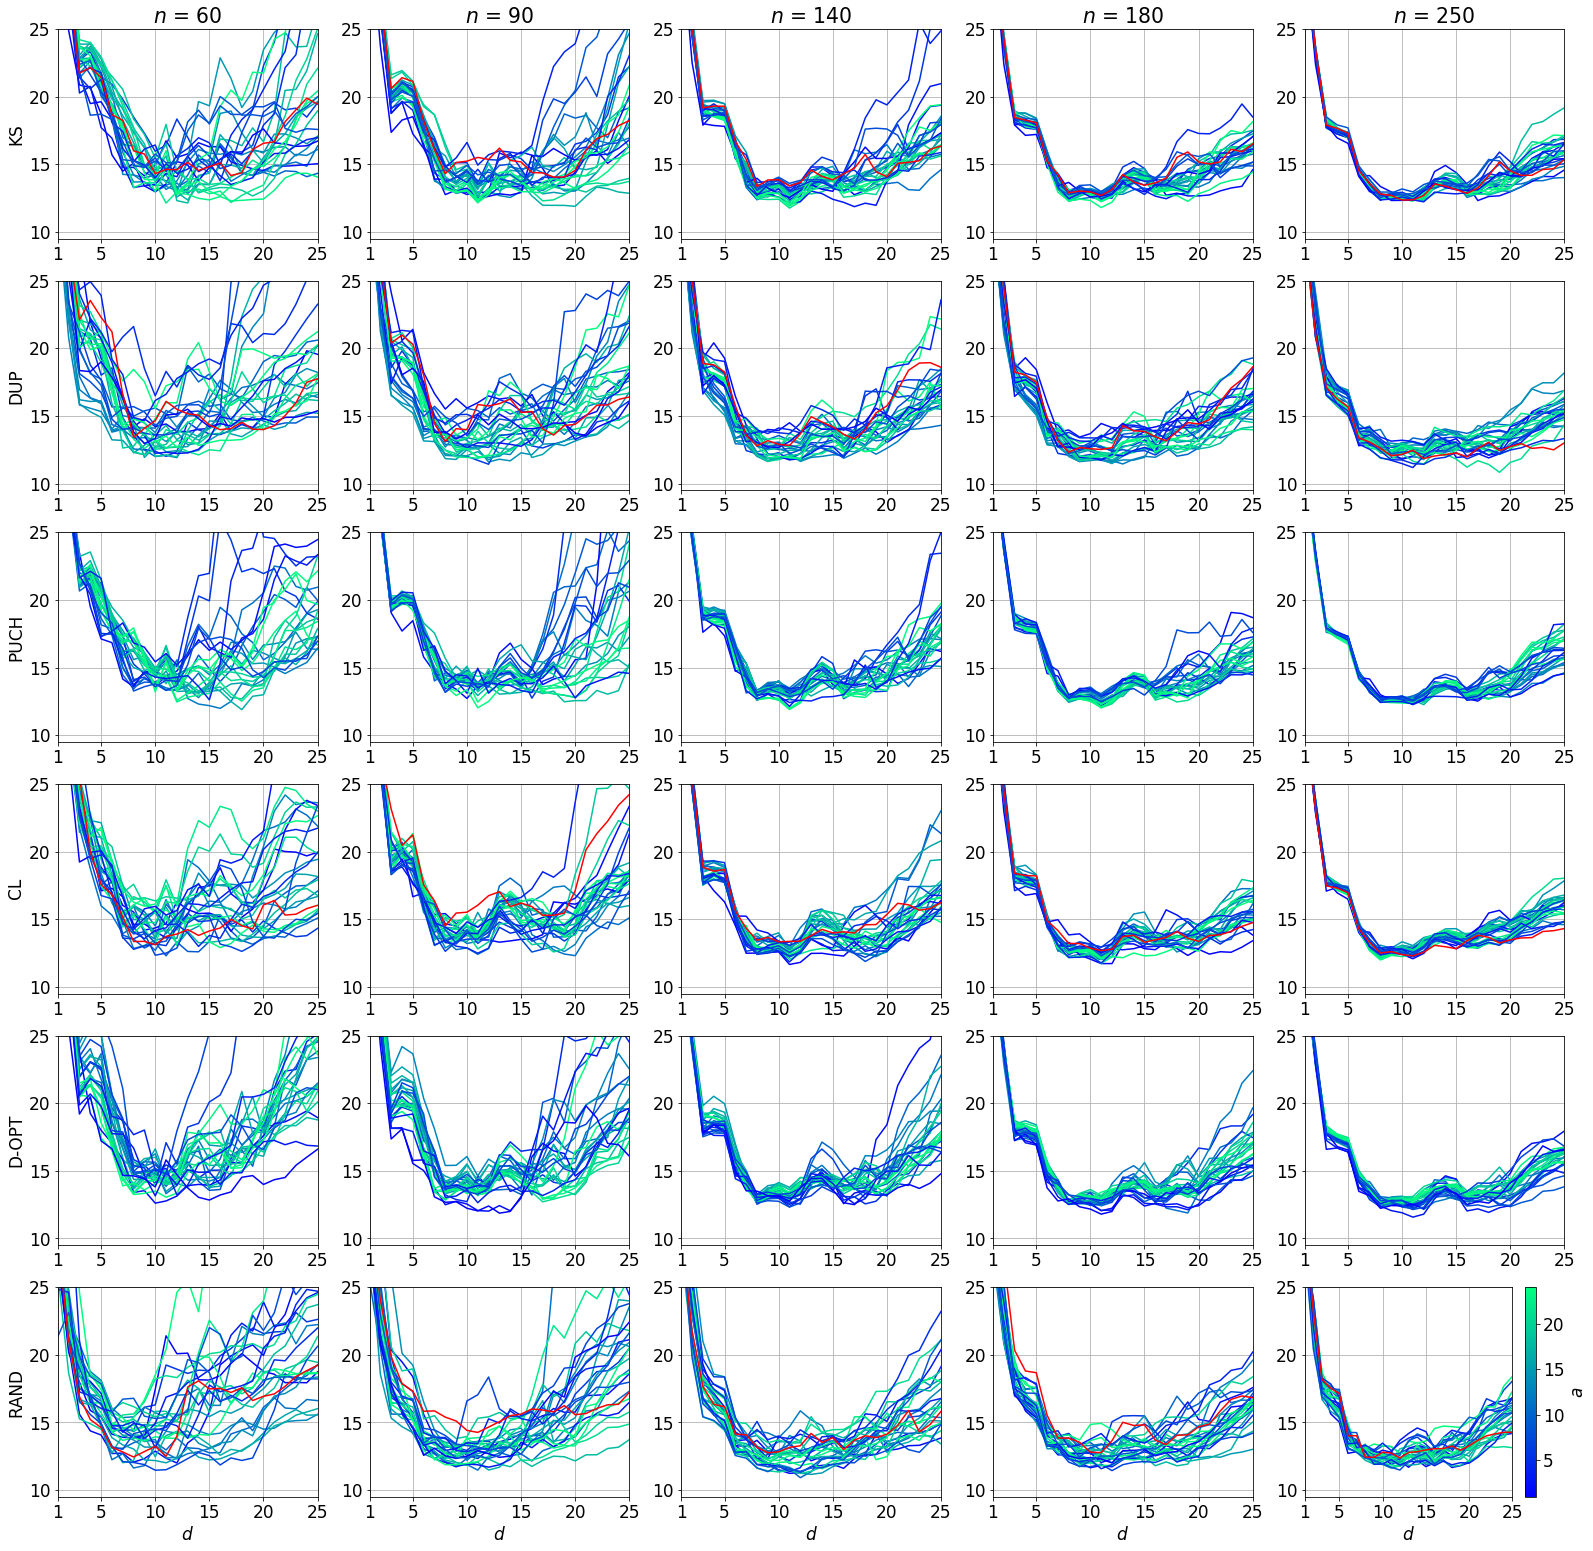
\includegraphics[width=0.8\textwidth]{manuscript/figures/d02_manure_model_performance.png}
\centering
\caption{Model performance to predict DM according to selection method, input dimensionality and sample size. The red line represents input dimensionality $a=p$.}
\label{fig_d02_manure_model_performance}
\end{figure}

% -----------------------------------------------------
% ------------------- discussion  ------------
% -----------------------------------------------------



\section*{Discussion}\label{discussion}

When positioning the PLSR algorithm in the general framework of statistical learning theory, it was found that the sample size needed to be establish multivariate calibration models is determined by the $VC$ dimension (i.e. model complexity). This means that a different sample size $n$ will be required for an easy-to-predict dominant chemical constituent than for a minor constituent that is harder to predict. This was revealed by the analysis of the ratio $n/d$ and the optimal sample sizes obtained in each case study. The level of easiness to predict is what the $VC$ dimension or model complexity represents. It was confirmed that a ratio $n/d>20$ accounts for a sample size that is rather large for a satisfactory calibration model. Based on the results of the present study, for which a hard-to-predict component (lactose in milk) and an easier component (dry matter in manure) were analyzed, evidence was obtained that a satisfactory calibration model can be built with $n/d>12$. While unsupervised sample selection is performed at a stage when no data on the target variable $y$ is available yet, it may be possible to estimate $d$ based on the literature and expert knowledge on the problem at hand.

In Au (2020)\cite{Au2020}, thresholds for the optimal sample size were found in absolute numbers. For the optimal complexity of 7 to 10 latent variables reported in that study, the found thresholds for the sample sizes correspond to ratios $n/d > 20$. Given that the sample size steps were taken larger, those results still confirm the theory based on the $n/d$ given by Vapnik \cite{Vapnik2000}.

The leading feature to address the current problem is that of spanning as much as possible the variability contained in the available selection set so that a representative subset of samples is obtained. In the context of chemometrics, this feature has not been concretely translated into a mathematical criterion, which at the same time is to be defined based on the model architecture that best describes the relationship between $\mathbf{X}$ and $y$. The specific framework analysis shows the role that the matrix $\mathbf{S}$ plays in the PLSR model, making it the mathematical element that can be controlled in an unsupervised setting. Therefore, finding a subset of $n$ samples that renders $\mathbf{S}_n$ equivalent to $\mathbf{S}_N$ has been proposed here as a way to define the representativity of the selected samples. 

The results obtained for the comparison of eigenvectors and eigenvalues showed that, provided the input dimensionality of $\mathbf{S}$, there is convergence in the equivalence of these matrices. Naturally, this equivalence depends on the input dimensionality $a$. For the purpose of PLSR model building, the value of $a$ needs to be higher than $d$ and it can be increased up to a value for which equivalence is supported by the fixed sample size based on $n/d>12$. In this way, as many PC dimensions of small variability as possible will be represented by the selected calibration set. From the model performance results obtained when selecting the samples based on a low input dimensionality (i.e. low number of PC's), it became clear that this may greatly compromise the performance of the model after gathering reference analyses. This insight was supported by the model performance achieved with high values of $a$ at least for KS, CL, PUCH and D-OPT and the high correlations between PC dimensions of low variability and $y$ in both case studies. While different researchers have reported to reduce the dimensionality for unsupervised sample selection, no general analysis of the effect of this dimensionality reduction was found \cite{Naes1990, Brandmaier2012, Nawar2018, Au2020}. On the other hand, it is not conclusive that selecting the samples with the original dimensionality of $\mathbf{X}$ was not found to be particularly advantageous over reducing it to $a<<p$. This is relevant for D-OPT which does not support the original matrix $\mathbf{X}$ when its rank is deficient.

In our study, the effect of the selection method was largely diminished once the sample size and the dimensionality $a$ had been set. Nonetheless, each of the selection methods operates under their own criterion to span the variability. DUP is the least suitable method for unsupervised sample selection as it has been designed to separate the set into two equal subsets containing 50\% of the samples. It functions by finding two replicate submatrices in the matrix $\mathbf{X}$, which might not be the ideal separation according to the threshold for the optimal sample size as confirmed by the presented results. D-OPT selection, on the other hand, proved to consistently deliver an optimal selection for values of $a>15$, which are considered high provided that less than 10 PC's account for more than 95\% of the variability of $\mathbf{X}$. This method, however, is characterized by overestimating the variability, representing a possible challenge in presence of bad outliers or an advantage for good leverage points. CL demonstrates to be the most robust strategy for sample selection although it represents a risk when the sample size $n$ does not correspond to $n$ well-defined groups existing in the original set. This latter insight was hypothesized based on the drop of the determinant rendered by CL in both case studies. CL, KS and PUCH delivered representative calibration sets, but the results on model performance showed that this aspect is highly dependent on punctual values of the dimensionality $a$, rather than ranges of it. Therefore, a suitable selection criterion would then be one that, provided a rank $a$, delivers a set for which $\mathbf{S}_n$ and $\mathbf{S}_N$ are equivalent in terms of their eigenvectors and eigenvalues, subject to a ratio of the eigenvalues above 1 and as uniform as possible across the ED directions.

An important feature that is of question when using D-OPT selection is the so-called \emph{effects} to include, concretely, the polynomial degree of the input variables \cite{Goos2011}. When including only the main effects, D-OPT unavoidably selects the outer layer of the data variability. The inclusion of higher-order effects is justified on the assumption of nonlinear effects of the input variables for the response variable. As this assumption was not made in the current study and strong nonlinear effects would suggest another model architecture, no higher-order effects were included when using D-OPT sample selection.

Many researchers apply specific data preprocessing techniques to remove certain sources of uninformative variation from the signals. Possible advantages of preprocessing the spectral data prior to unsupervised sample selection have been reported \cite{Liu2019}. However, initial experiments in the current case studies suggested that assuming advanced preprocessing such as scatter correction resulted in sets rendering calibration models with poor performance. This suggests that strong assumptions related to the required preprocessing prior to obtaining reference analyses are not recommended.

% -----------------------------------------------------
% ------------------- a scheme  ------------
% -----------------------------------------------------

\section*{A guideline for selecting the most informative calibration samples}\label{scheme}

The proposed guideline is visualized in Figure \ref{fig_scheme}. The higher mentioned conclusions from the exhaustive comparison of the factors involved in unsupervised sample selection can be summarized in a guideline for the establishment of multivariate calibration models. After defining the maximum value for the PLSR model complexity $d$ based on expert knowledge and literature, the optimal sample size $n$ can be calculated as 12$*d+1$. Once $n$ has been calculated, a value for the input dimensionality $a$ can be found by evaluating at what value of $a>d$ there is convergence in equivalence between $\mathbf{S}_N$ and $\mathbf{S}_n$. This ensures that the dimensions included in the selection account for PC's of small variability that can be beneficial for the PLSR model if a hard-to-predict constituent is involved. The samples can be selected with KS, PUCH, CL or D-OPT, evaluating which method delivers the best equivalence of the covariance matrices based on their eigendecompositions. It is recommended to analyze the presence of potential outliers, in particular when using D-OPT selection. In presence of outliers, the selection can be made replacing classical PCA for robust PCA \cite{Hubert2005}.


\begin{figure}[b]
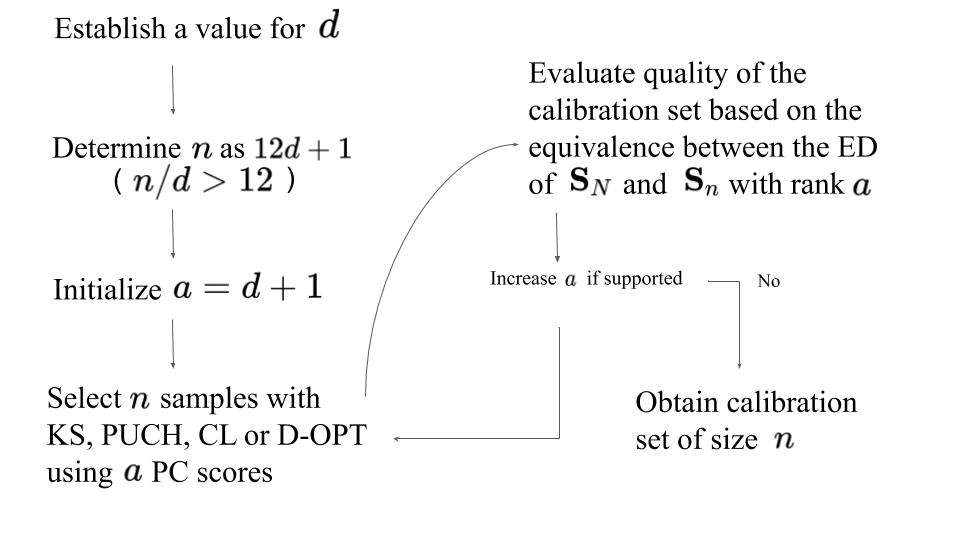
\includegraphics[width=0.6\textwidth]{manuscript/figures/scheme.png}
\centering
\caption{Proposed scheme for unsupervised sample selection in multivariate calibration}
\label{fig_scheme}
\end{figure}

% -----------------------------------------------------
% ------------------- conclusions  ------------
% -----------------------------------------------------

\section*{Conclusions}\label{conclusions}

The positioning of PLSR models in the general framework of statistical learning theory allowed to establish an objective threshold for the optimal sample size to build this type of calibration models. It was demonstrated that the input dimensionality $a$ plays an important role in the challenge of unsupervised sample selection and that PC dimensions of low variability still count for informative samples depending on the dominance of the target chemical constituent. The selection methods that have been a standard for sample selection for multivariate calibration proved to be equally useful for this challenge after controlling the sample size and the input dimensionality. RAND selection was found to be equally applicable for large sample sizes. 

The proposed scheme was developed in the context of PLSR models. However, most model architectures, including nonlinear models such as neural networks or support vector machines relate to a $VC$ dimension which can be theoretically determined or practically estimated \cite{Vapnik2019, Vapnik1994}. This is also not restricted only to regression models, the same ideas apply for classification models. This means that optimal sample sizes can be calculated based on the ratio $n/d$ if an estimation on the model complexity $d$ can be found for the problem at hand. 

The criterion based on the equivalence between $\mathbf{S}_N$ and $\mathbf{S}_n$ is specific for the PLSR model architecture or similar models such as PLS discriminant analysis, linear regression, among others. For every model architecture, it is advisable to identify the mathematical components that could be controlled in unsupervised sample selection \cite{Li2020}. 


Future work: refining of the criterion for Sn and SN equivalence and computational implementation in case a clear criterion can be defined. Dissemination of this type of analysis as it is the most accurate for unsupervised selection

% -----------------------------------------------------
% ------------------- data availability  ------------
% -----------------------------------------------------

\section{Data availability}

All the methodology that was used in the present work is available for public share. 

% -----------------------------------------------------
% ------------------- acknowledgements  ------------
% -----------------------------------------------------

\begin{acknowledgement}

Valeria Fonseca Diaz is funded as aspirant to doctoral fellow of
the Research Foundation-Flanders (FWO Brussels, Belgium).
The authors thank Dr. Raffaele Vitale and professor Peter Goos (KU Leuven, Belgium) for their suggestions on the conducted analysis given their expertise in Chemometrics and Experimental Design. 
\end{acknowledgement}

% -----------------------------------------------------
% ------------------- bibliography  ------------
% -----------------------------------------------------



\bibliography{biblio}


\end{document}

